% !TEX program = xelatex
% NC-format manuscript (bilingual Chinese-English)
% Compile: xelatex manuscript_bilingual.tex
\documentclass[11pt,a4paper]{article}

\usepackage[margin=2.4cm]{geometry}
\usepackage{xeCJK}
\usepackage{amsmath,amssymb}
\usepackage{graphicx}
\usepackage{setspace}
\usepackage{parskip}
\usepackage{titlesec}
\usepackage{booktabs}
\usepackage{tabularx}
\usepackage{multirow}
\usepackage{hyperref}
\usepackage{xcolor}
\usepackage{caption}

\setCJKmainfont{PingFang SC}[AutoFakeBold=true]
\setmainfont{Times New Roman}

\titleformat{\section}{\normalfont\large\bfseries}{\thesection}{0.6em}{}
\titleformat{\subsection}{\normalfont\normalsize\bfseries}{\thesubsection}{0.5em}{}

\setlength{\parskip}{0.6em}
\setlength{\parindent}{0pt}
\onehalfspacing

% Figure path
\graphicspath{{../../0414_v4/figures/}}

% Convenience macros
\newcommand{\keff}{\ensuremath{k_{\mathrm{eff}}}}
\newcommand{\Eint}{\ensuremath{E_{\mathrm{intercept}}}}
\newcommand{\Eslope}{\ensuremath{E_{\mathrm{slope}}}}
\newcommand{\abase}{\ensuremath{\alpha_{\mathrm{base}}}}
\newcommand{\aslope}{\ensuremath{\alpha_{\mathrm{slope}}}}
\newcommand{\kref}{\ensuremath{k_{\mathrm{ref}}}}
\newcommand{\Tref}{\ensuremath{T_{\mathrm{ref}}}}
\newcommand{\kslope}{\ensuremath{k_{\mathrm{slope}}}}

\title{\textbf{Bayesian Neural Surrogates Unify Uncertainty Propagation,\\
Sensitivity Attribution and Calibration for Coupled\\
Multi-Physics Reactor Analysis}\\[0.4em]
\large 贝叶斯神经代理统一耦合多物理反应堆分析中的\\
不确定性传播、敏感性归因与标定}
\author{Yinuo Chen\textsuperscript{1,2},
Sicheng Wang\textsuperscript{2,3},
Xiaojing Liu\textsuperscript{1,2},
Tengfei Zhang\textsuperscript{1,2*}\\[0.5em]
\small 1.~School of Nuclear Science and Engineering, Shanghai Jiao Tong University,
Shanghai 200240, China\\
\small 2.~Shanghai Digital Nuclear Reactor Technology Integration Innovation Center,
Shanghai 200240, China\\
\small 3.~College of Smart Energy, Shanghai Jiao Tong University,
Shanghai 200240, China\\[0.3em]
\small *~Corresponding author: \texttt{zhangtengfei@sjtu.edu.cn}}
\date{NC Draft (bilingual) \textperiodcentered{} \today}

\begin{document}
\maketitle

% ======================================================================
\section*{Abstract / 摘要}
% ======================================================================

We train a Bayesian neural network (BNN) surrogate on coupled
OpenMC--FEniCS data of a heat-pipe-cooled microreactor and use its
posterior predictive distribution as the single probabilistic object on
which forward uncertainty propagation, Sobol sensitivity attribution and
MCMC posterior calibration all operate, without retraining or
recalibration between analyses. Two-way neutronic--thermal--structural
coupling damps stress variability by approximately 30\% relative to a
decoupled prediction; stress and reactivity are governed by largely
separate material parameters (\Eint{} and \abase{}, respectively); and
across 18 benchmark calibrations the posterior contracts toward
observation-compatible regions with 90\%-CI coverage of 0.861. Each
posterior predictive draw costs approximately $1.43\times 10^{5}$ times
less than a coupled high-fidelity solve, enabling the full uncertainty
workflow to run end-to-end on a single workstation. The
posterior-predictive framework is directly applicable to other coupled
multi-physics systems.

本文在耦合 OpenMC--FEniCS 热管冷却微型反应堆数据上训练贝叶斯神经网络
（BNN）代理，以其后验预测分布作为前向不确定性传播、Sobol 敏感性归因
与 MCMC 后验标定三类分析共用的概率对象，三者之间无需各自重训或重新
校准。双向中子--热--力耦合使应力变异相对解耦预测降低约 30\%；应力与
反应性分别由杨氏模量截距（\Eint{}）与热膨胀系数（\abase{}）主导；在
18 例基准标定中，后验分布收敛至与观测相容的区域，90\%-CI 覆盖率为
0.861。每次后验预测抽样的代价较耦合高保真求解降低约
$1.43\times 10^{5}$ 倍，完整的不确定性工作流可在单台工作站上端到端
运行。该后验预测框架可直接推广至其他耦合多物理系统。

% ======================================================================
\section{Introduction / 引言}
% ======================================================================

Microreactors---compact, transportable fission systems rated at
1--20\,MW$_\mathrm{e}$---are being developed for decentralized power
generation in remote communities, defense installations and space
missions\textsuperscript{1,11}. NASA and DOE are advancing fission
surface-power systems for sustained lunar and planetary
operations\textsuperscript{12}, while rapidly growing electricity demand
from AI-intensive data centres reinforces the case for distributed,
dispatchable zero-carbon generation\textsuperscript{13}. Unlike
conventional large-scale plants, these designs concentrate fission power,
heat removal and structural loading within a compact monolithic core
where neutronics, heat transfer and structural mechanics are tightly
coupled through two-way feedback\textsuperscript{1,2}. A single
uncertain material parameter can simultaneously alter the neutronic
balance, the thermal field and the stress state; the closed feedback
loop may amplify or damp the resulting variability in ways that
single-physics analyses cannot capture. The uncertainty problem in these
systems is therefore inherently coupled.

微型反应堆——额定 1--20\,MW$_\mathrm{e}$ 的紧凑、可运输裂变系统——正面向
偏远社区、国防设施及太空任务中的分布式供能而开发\textsuperscript{1,11}。
NASA 与 DOE 正推进月面及行星任务的裂变地表供电系统\textsuperscript{12}，
与此同时 AI 密集型数据中心电力需求的快速增长进一步强化了分布式、
可调度零碳发电的需求\textsuperscript{13}。与常规大型电厂不同，
此类设计将裂变功率、热量排出与结构载荷集中于紧凑的一体式堆芯，
中子学、传热与结构力学通过双向反馈紧密耦合\textsuperscript{1,2}。
单个不确定材料参数可同时改变中子平衡、温度场与应力状态；闭合反馈回路
可能以单物理分析无法捕捉的方式放大或衰减由此产生的变异。因此，
此类系统的不确定性问题本质上是耦合的。

High-fidelity coupled solvers now exist for these systems: MOOSE-based
toolchains handle neutronics--thermo-mechanics--heat-pipe coupling for
KRUSTY-class and larger designs\textsuperscript{2,3}, and
thermal--structural analyses have established stress concentration as a
persistent safety concern in monolithic-core
configurations\textsuperscript{4,5}. Surrogate-assisted probabilistic
modules in the MOOSE ecosystem\textsuperscript{6,7} and digital-twin
pipelines\textsuperscript{8} address forward propagation, sensitivity or
calibration individually, but each uses a separately constructed model
with no shared probabilistic basis between analyses.

高保真耦合求解器已适用于这类系统：基于 MOOSE 的工具链可处理 KRUSTY 类
及更大设计上的中子--热力--热管耦合\textsuperscript{2,3}；热--力分析已确认
应力集中是一体式堆芯构型中持续性的安全关注\textsuperscript{4,5}。
MOOSE 生态\textsuperscript{6,7} 与数字孪生管线\textsuperscript{8}
中的代理辅助概率模块分别处理前向传播、敏感性或标定，但每类分析各自
构建独立模型，三者之间缺乏共享的概率基础。

Running the full probabilistic workflow---forward uncertainty
propagation, global sensitivity analysis and Bayesian
calibration---directly on the coupled solver is impractical at
${\sim}10^{3}$\,s per solve. Gaussian-process and polynomial-chaos
surrogates face dimensionality constraints in nonlinear coupled settings;
physics-informed neural networks require a closed residual form that
iterative solver exchange does not supply; deterministic neural networks
produce only point predictions. None of these provides the coherent
predictive distribution that all three analyses require.

在耦合求解器上直接运行完整的概率工作流——前向不确定性传播、全局
敏感性分析与贝叶斯标定——不可行，每次求解约需 $10^{3}$\,s。高斯过程
与多项式混沌代理在非线性耦合设置下受维度限制；物理信息神经网络需要
闭合残差形式，而迭代求解器交换无法提供；确定性神经网络仅产生点估计。
上述方案均无法提供三类分析共同所需的连贯预测分布。

A Bayesian neural network (BNN) fills this gap. By placing a
distribution over the network weights, a BNN yields a posterior
predictive distribution that can be sampled at negligible cost once
trained. This single distribution serves as the shared probabilistic
layer on which forward propagation, variance-based sensitivity
attribution and observation-conditioned posterior calibration all
operate, with no retraining or recalibration between them.

贝叶斯神经网络（BNN）填补了这一空缺。通过对权重引入分布，BNN 在
训练完成后即可以极低代价反复采样其后验预测分布。该分布充当前向传播、
基于方差的敏感性归因与观测条件后验标定共同使用的概率层，三者之间无需
重训或重新校准。

This paper presents a BNN-based posterior-predictive framework for
end-to-end probabilistic analysis of coupled multi-physics systems. The
framework unifies forward uncertainty propagation, Sobol sensitivity
decomposition and MCMC posterior calibration on a single predictive
layer trained on coupled OpenMC--FEniCS data of a heat-pipe-cooled
reactor. It reveals that two-way coupling damps stress variability by
approximately 30\%, that stress and reactivity are governed by largely
separate parameter pathways, and that the posterior calibration contracts
the material-parameter distribution toward observation-compatible
regions---all at five orders of magnitude less cost per evaluation
than a coupled high-fidelity solve.

本文提出了一套基于 BNN 后验预测分布的耦合多物理系统端到端概率分析
框架。该框架将前向不确定性传播、Sobol 敏感性分解与 MCMC 后验标定统一
到基于热管冷却反应堆耦合 OpenMC--FEniCS 数据训练的单一预测层上。框架
揭示：双向耦合使应力标准差相对解耦预测降低约 30\%；应力与反应性分别受制于基本独立
的参数通道；后验标定将材料参数分布收敛至与观测相容的区域——以上分析
的单次评估代价较耦合高保真求解低约五个数量级。

% ======================================================================
\section{Results / 结果}
% ======================================================================

\subsection{Surrogate accuracy and calibration / 代理精度与校准}

The framework rests on a single BNN that predicts all 15 coupled and
decoupled outputs simultaneously; if this surrogate is inaccurate, the
downstream propagation, sensitivity and calibration results are
unreliable. We evaluated the physics-regularized BNN alongside a
reference (unconstrained) BNN and two conventional baselines---MC-Dropout
and a five-member deep ensemble---on 501 held-out test samples (Table~1,
Fig.~1). Results for the physics-regularized BNN are reported as
mean $\pm$ s.d.\ across 5 random seeds; ablation across both BNN
variants is in Supplementary Table~S3.

该框架依赖一个同时预测全部 15 个耦合与解耦输出的 BNN；若代理精度不足，
下游的传播、敏感性与标定结论均不可靠。我们将物理正则化 BNN 与参考
（无约束）BNN 及两种传统基线方法——MC-Dropout 和五成员深度集成——在
501 个留出测试样本上进行了评估（表~1，图~1）。物理正则化 BNN 的结果以
5 个随机种子的均值 $\pm$ 标准差报告；两种 BNN 变体的消融实验见补充表~S3。

On coupled peak global stress the physics-regularized BNN achieves
$R^2 = 0.935 \pm 0.007$ (RMSE $7.63 \pm 0.47$\,MPa), comparable to
MC-Dropout ($R^2 = 0.934$) and deep ensemble ($R^2 = 0.934$). The BNN
advantage is most pronounced on temperature outputs: for maximum fuel
temperature the BNN RMSE is $4.26 \pm 0.18$\,K versus 4.50\,K for both
baselines, and the expected calibration error (ECE) is 0.027 versus
0.183 (MC-Dropout) and 0.190 (deep ensemble)---a five- to six-fold
improvement in calibration quality (Fig.~1A,~C).

在耦合峰值全局应力上，物理正则化 BNN 达到
$R^2 = 0.935 \pm 0.007$（RMSE $7.63 \pm 0.47$\,MPa），与 MC-Dropout
（$R^2 = 0.934$）和深度集成（$R^2 = 0.934$）相当。BNN 的优势在温度
输出上最为显著：最大燃料温度的 BNN RMSE 为 $4.26 \pm 0.18$\,K，而
两种基线方法均为 4.50\,K；期望校准误差（ECE）为 0.027，而 MC-Dropout
为 0.183、深度集成为 0.190——校准质量提升五至六倍（图~1A、C）。

The 90\% predictive intervals are conservatively calibrated across all
outputs (PICP 0.937--1.000), and incorporating physics-prior monotonicity
constraints tightens the intervals relative to the unconstrained
reference without reducing coverage (Supplementary Table~S3). The
continuous ranked probability score (CRPS) is lowest for the
physics-regularized BNN on all five primary outputs (Table~1).

所有输出的 90\% 预测区间均呈保守校准特性（PICP 0.937--1.000），引入
物理先验单调性约束可在不降低覆盖率的前提下收窄区间（补充表~S3）。
在五个主要输出上，物理正则化 BNN 的连续排序概率评分（CRPS）均为
最低（表~1）。

\begin{figure}[htbp]
\centering
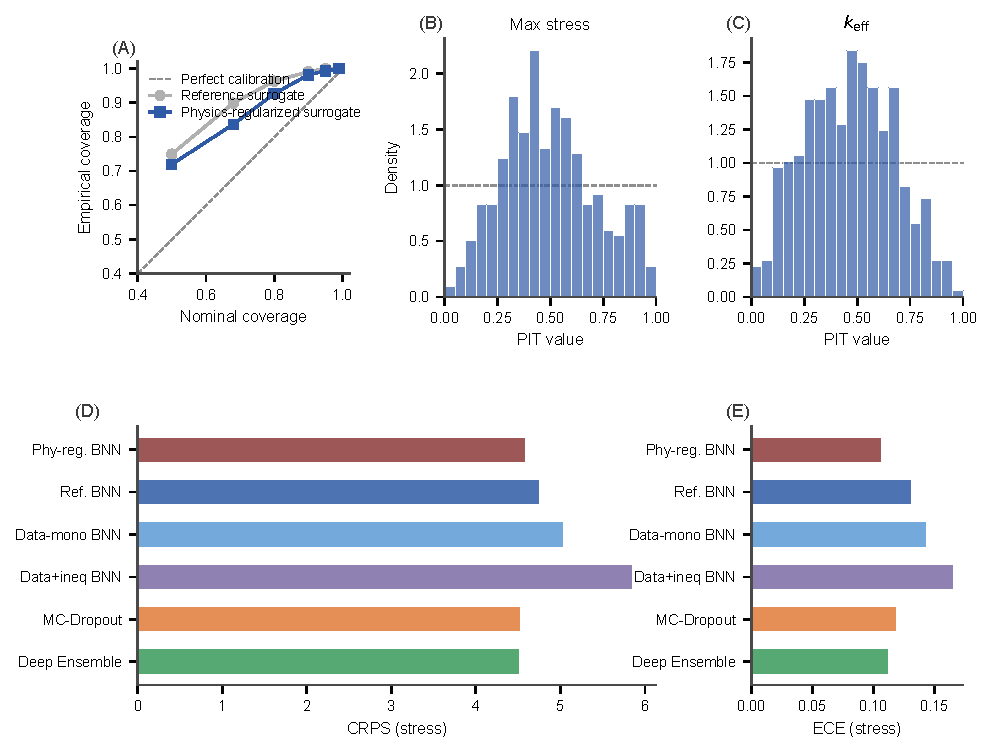
\includegraphics[width=\textwidth]{fig1_accuracy.pdf}
\caption{\textbf{Surrogate accuracy and uncertainty calibration.}
(\textbf{A})~Predicted vs.\ true values for five primary coupled outputs
(physics-regularized BNN, 501 test samples).
(\textbf{B})~Residual distributions.
(\textbf{C})~Calibration curves comparing BNN, MC-Dropout and deep
ensemble. The BNN achieves five- to six-fold lower ECE than the baselines
on temperature outputs.}
\label{fig:accuracy}
\end{figure}

% --- Table 1: Full accuracy comparison ---
\begin{table}[htbp]
\centering
\caption{\textbf{Surrogate accuracy on five primary coupled outputs.}
Physics-regularized BNN: mean $\pm$ s.d.\ across 5 seeds; external
baselines: single run. Bold CRPS indicates best per output.\\
\small 表~1~|~五个主要耦合输出的代理精度。物理正则化 BNN：5 个种子的
均值 $\pm$ 标准差；外部基线：单次运行。粗体 CRPS：各输出最优。}
\label{tab:accuracy}
\smallskip
\small
\begin{tabular}{lccccc}
\toprule
Output & $R^2$ & RMSE & PICP & ECE & CRPS \\
\midrule
\multicolumn{6}{l}{\textit{Physics-regularized BNN}} \\
\quad \keff{}
  & $0.633 \pm 0.258$
  & $0.0006 \pm 0.0004$
  & $0.981 \pm 0.007$
  & 0.123
  & \textbf{0.0002} \\
\quad Max.\ fuel temp.
  & $0.621 \pm 0.044$
  & $4.26 \pm 0.18$\,K
  & $0.936 \pm 0.015$
  & 0.027
  & \textbf{2.39} \\
\quad Max.\ monolith temp.
  & $0.622 \pm 0.044$
  & $4.80 \pm 0.20$\,K
  & $0.942 \pm 0.013$
  & 0.031
  & \textbf{2.70} \\
\quad Max.\ global stress
  & $0.935 \pm 0.007$
  & $7.63 \pm 0.47$\,MPa
  & $0.987 \pm 0.007$
  & 0.106
  & \textbf{4.58} \\
\quad Wall expansion
  & $0.993 \pm 0.001$
  & $0.0020 \pm 0.0002$
  & $1.000 \pm 0.000$
  & 0.194
  & \textbf{0.0017} \\
\midrule
\multicolumn{6}{l}{\textit{MC-Dropout}} \\
\quad Max.\ fuel temp.
  & 0.590  & 4.50\,K  & ---  & 0.183  & 2.62 \\
\quad Max.\ global stress
  & 0.934  & 7.66\,MPa  & ---  & 0.118  & 4.52 \\
\midrule
\multicolumn{6}{l}{\textit{Deep Ensemble (5 members)}} \\
\quad Max.\ fuel temp.
  & 0.590  & 4.49\,K  & ---  & 0.190  & 2.63 \\
\quad Max.\ global stress
  & 0.934  & 7.64\,MPa  & ---  & 0.112  & 4.50 \\
\bottomrule
\end{tabular}
\end{table}


\subsection{Physics consistency / 物理一致性}

We verified the BNN's adherence to known physical relationships through
two tests: monotonicity verification against 15 input--output pairs
derived from the constitutive laws, and ordering/non-negativity
constraint satisfaction (Fig.~2A). For all high-confidence monotonicity
pairs---including the dominant stress drivers \Eint{} (+), \abase{} (+),
and \kref{} ($-$)---both BNN variants achieved zero violation rates
on the 501 held-out test samples using discrete $\pm\delta$ perturbation
testing. The only non-trivial violations occurred for the
medium-confidence pair SS316\_$\alpha$ $\to$ fuel temperature (36--54\%
across models), reflecting a weaker and potentially nonlinear
relationship that the training data does not consistently support. All
four models also satisfied ordering constraints
(max $\geq$ average temperature) and non-negativity constraints
(stress $\geq 0$) with zero violations.

我们通过两项测试验证了 BNN 对已知物理关系的遵守情况：针对由本构方程
推导的 15 个输入--输出对进行单调性验证，以及排序/非负约束满足性测试
（图~2A）。对于所有高置信度单调对——包括应力的主要驱动因素
\Eint{}（+）、\abase{}（+）和 \kref{}（$-$）——两种 BNN 变体在 501 个
测试样本上通过离散 $\pm\delta$ 扰动测试均实现了零违反率。唯一的显著违反
出现在中等置信度的 SS316\_$\alpha$ $\to$ 燃料温度对（各模型 36--54\%），
反映了一种较弱且可能非线性的物理关系。两个模型在排序约束
（最大 $\geq$ 平均温度）和非负约束（应力 $\geq 0$）上均实现零违反。

Decomposing total predictive variance into epistemic
(weight-uncertainty) and aleatoric (observation-noise) components
revealed that aleatoric uncertainty dominates across all outputs,
accounting for 58--90\% of total variance (Fig.~2B). The epistemic
fraction was highest for wall expansion (${\sim}42\%$) and stress
(${\sim}30\%$), indicating greater model-form uncertainty for these
mechanically driven outputs.

将总预测方差分解为认知（权重不确定性）和偶然（观测噪声）分量后发现，
偶然不确定性在所有输出上占主导地位，占总方差的 58--90\%（图~2B）。
认知不确定性占比最高的是壁面膨胀（${\sim}42\%$）和应力
（${\sim}30\%$），表明模型对这些力学驱动输出的结构不确定性较大。物理
正则化略微降低了温度预测的认知不确定性（认知占比 10.1\%，而参考 BNN
为 11.2--12.0\%），这与单调性约束限制了可信模型结构空间的预期一致。

\begin{figure}[htbp]
\centering
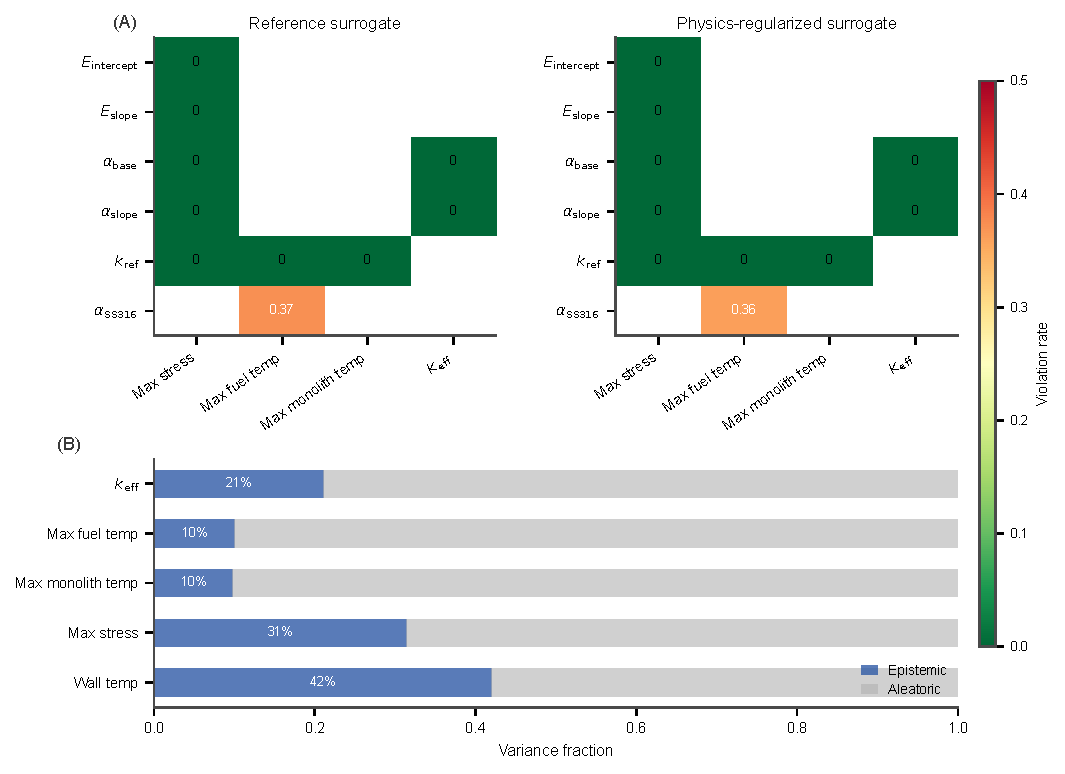
\includegraphics[width=\textwidth]{fig5_physics.pdf}
\caption{\textbf{Physics consistency verification.}
(\textbf{A})~Monotonicity violation rates for 15 input--output pairs
across both BNN variants; high-confidence pairs achieve zero violations.
(\textbf{B})~Epistemic vs.\ aleatoric variance decomposition across
five primary outputs.}
\label{fig:physics}
\end{figure}


\subsection{Forward uncertainty propagation / 前向不确定性传播}

Propagating 20,000 Latin hypercube samples through the BNN posterior
predictive mean yields a coupled stress distribution with mean
161.7\,MPa and standard deviation 31.9\,MPa, versus a decoupled mean of
203.5\,MPa and standard deviation of 45.6\,MPa. Coupling reduces the
stress standard deviation by approximately 30\% and lowers the mean by
approximately 42\,MPa (Table~2, Fig.~3).

将 20,000 个拉丁超立方采样点通过 BNN 后验预测均值传播，得到耦合应力
分布均值 161.7\,MPa、标准差 31.9\,MPa，而解耦分布均值为 203.5\,MPa、
标准差 45.6\,MPa。耦合使应力标准差降低约 30\%，均值降低约 42\,MPa
（表~2，图~3）。

The coupled \keff{} has mean 1.1036 and standard deviation approximately
77\,pcm. The decoupled \keff{} is effectively constant because, at the
reference geometry, the sampled material parameters do not enter the
neutronic cross-section tables; all coupled \keff{} variability
originates from thermal-expansion modification of core geometry.

耦合 \keff{} 均值为 1.1036，标准差约 77\,pcm。解耦 \keff{} 几乎恒定，
因为在参考几何下，采样的材料参数不进入中子截面表；耦合 \keff{} 的全部
变异源自热膨胀对堆芯几何的修改。

\begin{table}[htbp]
\centering
\caption{\textbf{Forward UQ summary: coupled vs.\ decoupled distributions}
(20,000 LHS samples through BNN posterior predictive mean).\\
\small 表~2~|~前向 UQ 汇总：耦合与解耦分布。}
\label{tab:forward}
\smallskip
\begin{tabular}{lcccc}
\toprule
Output & Coupled mean & Coupled s.d. & Decoupled mean & Decoupled s.d. \\
\midrule
Stress (MPa) & 161.7 & 31.9 & 203.5 & 45.6 \\
\keff{} & 1.1036 & 0.00077 & $\sim$constant & $\sim$0 \\
\bottomrule
\end{tabular}
\end{table}

\begin{figure}[htbp]
\centering
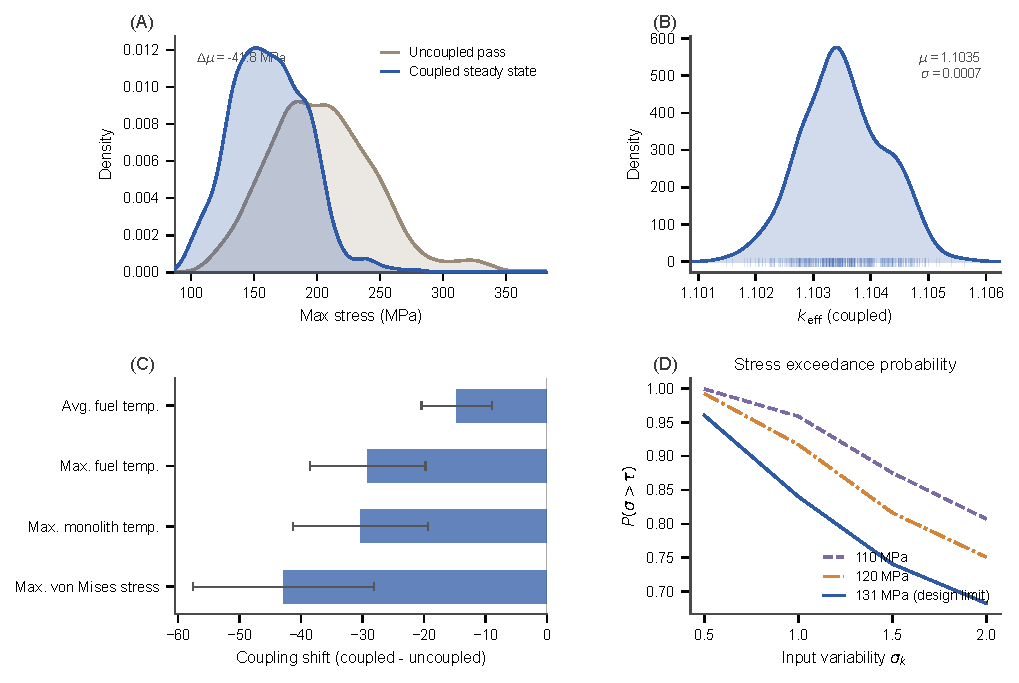
\includegraphics[width=\textwidth]{fig3_forward.pdf}
\caption{\textbf{Forward uncertainty propagation.}
Coupled vs.\ decoupled output distributions for stress and \keff{}.
Two-way coupling reduces the stress standard deviation by ${\approx}30\%$
and introduces \keff{} variability that is absent in the decoupled case.}
\label{fig:forward}
\end{figure}


\subsection{Global sensitivity analysis / 全局敏感性分析}

Sobol analysis (50 independent replications, $N_S = 4096$ per matrix;
full index table in Supplementary Table~S4) shows that stress and
\keff{} are governed by two largely separate physical pathways
(Table~3, Fig.~4).

Sobol 分析（50 次独立重复，每矩阵 $N_S = 4096$；完整指标表见补充
表~S4）表明应力与 \keff{} 受制于两条基本独立的物理路径（表~3，图~4）。

Stress is rooted in the elastic-constitutive pathway. \Eint{} alone
accounts for approximately 55\% of the first-order variance
($S_1 = 0.548$, 90\% CI [0.498, 0.572]), and the near-zero gap between
its total-order and first-order indices indicates that it acts with
minimal interaction. Secondary contributors---\abase{}
($S_1 = 0.210$), \kref{} and $\nu$---add a collective approximately
15\%, while the remaining parameters are negligible. The dominance of
\Eint{} is a direct consequence of the generalised Hooke's law:
stiffness enters the stress field linearly.

应力根植于弹性本构路径。\Eint{} 单独贡献约 55\% 的一阶方差
（$S_1 = 0.548$，90\% CI [0.498, 0.572]），其全阶与一阶指标之间的
差距接近零，表明其作用几乎无交互。次要贡献因素——\abase{}
（$S_1 = 0.210$）、\kref{} 和 $\nu$——合计约贡献 15\%，其余参数
可忽略。\Eint{} 的主导地位是广义胡克定律的直接结果：刚度线性进入
应力场。

\keff{} is rooted in the thermal-expansion pathway. \abase{} accounts
for approximately 77\% of the first-order variance
($S_1 = 0.771$, 90\% CI [0.747, 0.788]): it sets the magnitude of
geometric expansion, which alters neutron leakage and shifts the
neutronic balance. \aslope{} contributes a further approximately 19\%
($S_1 = 0.195$), while no elasticity or conductivity parameter has a
first-order effect on reactivity above the noise floor.

\keff{} 根植于热膨胀路径。\abase{} 贡献约 77\% 的一阶方差
（$S_1 = 0.771$，90\% CI [0.747, 0.788]）：它设定了几何膨胀的幅度，
进而改变中子泄漏并移动中子学平衡点。\aslope{} 进一步贡献约 19\%
（$S_1 = 0.195$），而弹性或热导率参数对反应性的一阶效应均在噪声底以下。

The two pathways share almost no dominant parameters. This separation
means that stress and \keff{} observations constrain different regions
of the material-parameter space---an important constraint for any
monitoring strategy that aims to reduce material-property uncertainty.

两条路径几乎不共享主导参数。该分离意味着应力与 \keff{} 的观测约束了
材料参数空间的不同区域——这对任何旨在降低材料属性不确定性的监测策略
而言是一个重要约束。

Convergence analysis confirmed that these rankings stabilised by
$N_S = 2048$, with standard deviations below 0.04 at the final sample
size of 8192 (Supplementary Fig.~S5). Both the reference and
physics-regularized BNN yielded consistent rankings, indicating that
the regularization does not distort the sensitivity structure.

收敛性分析表明，上述排名在 $N_S = 2048$ 时已趋于稳定，在最终样本量 8192
处标准差低于 0.04（补充图~S5）。参考 BNN 与物理正则化 BNN 给出了一致的
排名，表明正则化未扭曲敏感性结构。

\begin{table}[htbp]
\centering
\caption{\textbf{First-order Sobol indices $S_1$ for stress and \keff{}}
(physics-regularized BNN, $N_S = 4096$, 50 replications, 90\% CI).
Only factors with CI lower bound $> 0$ are shown.\\
\small 表~3~|~应力与 \keff{} 的一阶 Sobol 指标 $S_1$。仅列出 CI 下界 $> 0$ 的因素。}
\label{tab:sobol}
\smallskip
\begin{tabular}{lcc}
\toprule
Parameter & Stress $S_1$ [90\% CI] & \keff{} $S_1$ [90\% CI] \\
\midrule
\Eint{}   & 0.548 [0.498, 0.572] & --- \\
\abase{}  & 0.210 [0.171, 0.254] & 0.771 [0.747, 0.788] \\
$\nu$     & 0.063 [0.034, 0.097] & --- \\
\kref{}   & 0.065 [0.014, 0.118] & --- \\
\aslope{} & --- & 0.195 [0.112, 0.250] \\
\bottomrule
\end{tabular}
\end{table}

\begin{figure}[htbp]
\centering
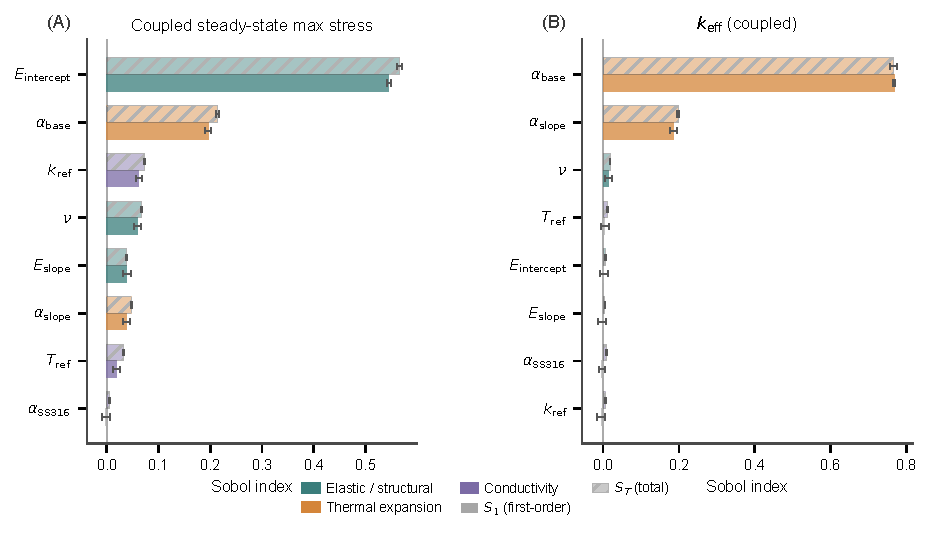
\includegraphics[width=\textwidth]{fig4_sobol.pdf}
\caption{\textbf{Sobol sensitivity analysis.}
First-order and total-order indices for stress and \keff{} reveal two
largely separate physical pathways: the elastic-constitutive pathway
(dominated by \Eint{}) for stress, and the thermal-expansion pathway
(dominated by \abase{}) for \keff{}.}
\label{fig:sobol}
\end{figure}


\subsection{Posterior calibration / 后验标定}

Bayesian calibration uses the same BNN to update the prior parameter
distribution given noisy observations. The four calibrated
parameters---\Eint{}, \abase{}, \aslope{} and \kref{}---are the four
that the Sobol analysis identified as covering the dominant variance
channels for stress and \keff{}. Metropolis--Hastings MCMC is run on 18
benchmark cases drawn from the test split (6 low / 6 near / 6 high
stress; details in Methods) with 4 independent chains per case.

贝叶斯标定利用同一 BNN 在给定含噪观测数据的条件下更新先验参数分布。
四个标定参数——\Eint{}、\abase{}、\aslope{} 和 \kref{}——是 Sobol
分析所识别的覆盖应力与 \keff{} 主要方差通道的因素。Metropolis--Hastings
MCMC 在 18 个基准算例（取自测试集：低应力 6 例 / 阈值附近 6 例 /
高应力 6 例，详见方法部分）上运行，每个案例使用 4 条独立链。

Chain convergence was assessed using rank-normalised split-$\hat{R}$
(Vehtari et al.\ 2021) and Geyer initial-positive-sequence effective
sample size. Across all 72 parameter--case combinations for the
physics-regularized BNN, $\hat{R}_{\max} = 1.017$ (well below the 1.1
threshold), $\mathrm{ESS}_{\min} = 352$, and mean acceptance rate
$= 0.605$ (Fig.~5A--B; Supplementary
Table~S5).

链收敛性通过秩归一化 split-$\hat{R}$（Vehtari 等，2021）和 Geyer 初始正
序列有效样本量进行评估。在物理正则化 BNN 的全部 72 个参数--案例组合中，
$\hat{R}_{\max} = 1.017$（远低于 1.1 阈值），$\mathrm{ESS}_{\min} = 352$，
平均接受率 $= 0.605$（图~5A--B；补充表~S5）。

Across the 18 cases, the posterior 90\%-CI coverage is 0.861---the
observations successfully constrain the parameters that the Sobol
analysis flagged as most influential. In higher-stress cases, the
\Eint{} marginal shifts toward larger values, consistent with its
dominant role in the elastic-constitutive pathway. The joint posterior of
\Eint{} and \abase{} develops a compensation ridge: an increase in
stiffness can be partially offset by a decrease in thermal expansion,
leaving the stress product $\sigma \sim E \cdot \alpha \cdot \Delta T$
approximately invariant. This partial non-identifiability arises from
the multiplicative structure and would not be visible in a single-output
calibration (Fig.~5).

18 例的后验 90\%-CI 覆盖率为 0.861——观测数据成功约束了 Sobol 分析标记
为最具影响力的参数。在高应力算例中，\Eint{} 的边缘分布向更大值
偏移，这与其在弹性本构路径中的主导作用一致。\Eint{} 与 \abase{}
的联合后验形成补偿脊：刚度的增加可被热膨胀的降低部分抵消，使应力乘积
$\sigma \sim E \cdot \alpha \cdot \Delta T$ 近似不变。这种部分不可辨识性
源于乘法结构，在单输出标定中不可见（图~5）。

At the posterior-mean parameters of each case, the BNN-predicted stress
tracks the true value with MAE $= 10.4$\,MPa over a true-stress range
of 102--198\,MPa. Prior sensitivity analysis (6 prior configurations)
and observation noise sensitivity analysis (noise fraction 0.5--10\%)
confirmed the robustness of posterior inference (Supplementary
Figs.~S7--S8, Tables~S11--S12).

在各算例的后验均值参数处，BNN 预测应力跟踪真实值的 MAE $= 10.4$\,MPa，
真实应力范围为 102--198\,MPa。先验敏感性分析（6 种先验配置）和观测噪声
敏感性分析（噪声分数 0.5--10\%）确认了后验推断的鲁棒性（补充图~S7--S8，
补充表~S11--S12）。

\begin{figure}[htbp]
\centering
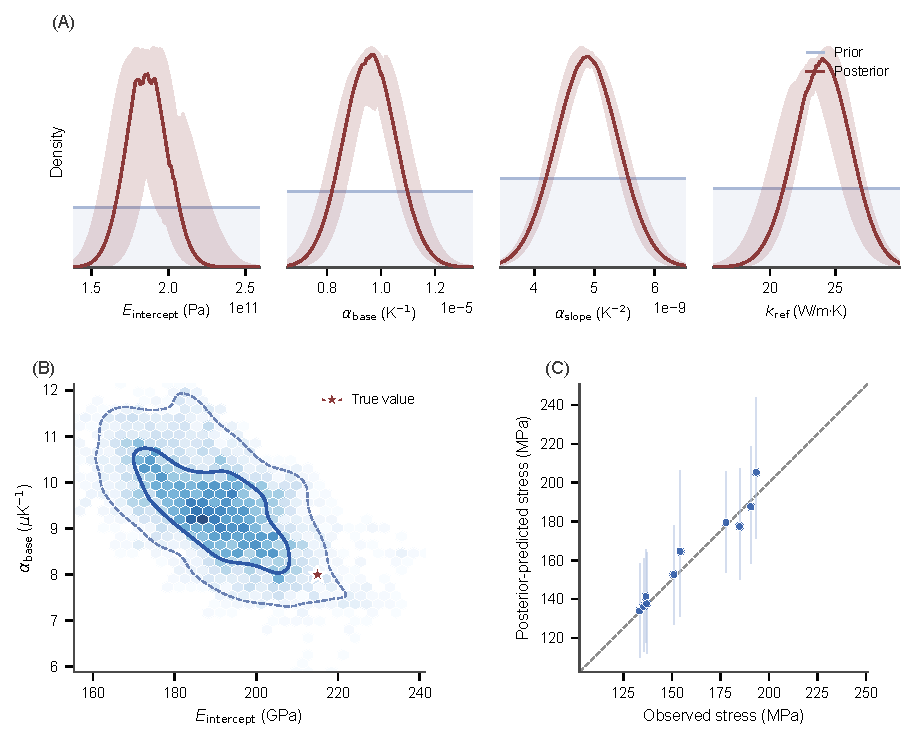
\includegraphics[width=\textwidth]{fig6_posterior.pdf}
\caption{\textbf{Posterior calibration results.}
(\textbf{A})~MCMC convergence diagnostics (split-$\hat{R}$ and ESS).
(\textbf{B})~Acceptance rates across 18 benchmark cases.
(\textbf{C})~Marginal posterior distributions for \Eint{} and \abase{}
in representative low-, near-, and high-stress cases.
(\textbf{D})~Joint posterior of \Eint{} vs.\ \abase{} showing the
compensation ridge.}
\label{fig:posterior}
\end{figure}


% ======================================================================
\section{Discussion / 讨论}
% ======================================================================

\subsection{Coupling feedback and uncertainty compression /
耦合反馈与不确定性压缩}

The stress standard deviation drops from approximately 45.6\,MPa in the
decoupled response to approximately 31.9\,MPa after coupling
convergence, a roughly 30\% reduction. The mechanism is the negative
neutronic--thermal feedback characteristic of compact monolithic-core
systems: thermal expansion modifies the core geometry, which shifts the
neutronic balance and partially offsets the direct stress increase. What
the BNN-based forward propagation establishes is the net effect of this
feedback on the output distribution. A decoupled analysis does not see
the feedback loop and therefore overestimates the parameter-driven stress
variability.

应力标准差从解耦响应的约 45.6\,MPa 降至耦合收敛后的约 31.9\,MPa，降幅
约 30\%。其机制是紧凑型一体式堆芯系统特有的负中子--热反馈：热膨胀修改
堆芯几何，移动中子学平衡点，从而部分抵消直接的应力增加。基于 BNN 的
前向传播所建立的是该反馈对输出分布的净效应。解耦分析无法感知反馈回路，
因而高估了参数驱动的应力变异。

The overestimate is conservative for safety-margin evaluation and cannot
produce an unsafe conclusion, but it inflates the apparent penalty of
material-property uncertainty. In practice, this can translate into
manufacturing tolerances stricter than the coupled response warrants.

这种高估对安全裕度评估而言是保守的，不会导致不安全的结论，但会放大
材料属性不确定性的表观代价。在工程实践中，这可能转化为比耦合响应所需
更严格的制造公差。

\subsection{BNN calibration and model selection /
BNN 校准与模型选择}

Both the unconstrained baseline and the physics-prior surrogate achieve
zero monotonicity violations on the test set. Incorporating
physics-prior monotonicity constraints modestly tightens predictive
intervals without reducing coverage (stress CRPS $4.42 \to 4.35$;
full ablation and small-sample data-efficiency analysis in
Supplementary Notes~G and~H). The same posterior predictive
distribution propagates consistently through forward UQ, Sobol
attribution and MCMC calibration---a point-estimate surrogate would
require separate uncertainty wrappers for each analysis with no
guarantee of mutual consistency. Heteroscedastic noise modelling is
retained over a homoscedastic alternative (Supplementary Note~H).

基线模型与物理先验代理在测试集上均未出现单调性违反。引入物理先验
单调性约束可在不降低覆盖率的前提下适度收紧预测区间（应力 CRPS
$4.42 \to 4.35$；完整消融与小样本数据效率分析见补充说明~G 与~H）。
同一后验预测分布在前向 UQ、Sobol 归因与 MCMC 标定之间一致传播——
点估计代理则需为每类分析分别构建不确定性包装器，且无法保证相互一致。
异方差噪声建模优于同方差替代方案（补充说明~H）。

Out-of-distribution analysis confirms that the BNN's epistemic
uncertainty inflates appropriately in under-represented input regions:
epistemic standard deviation increases by 7--21\% in peripheral-tail
subsets, while 90\% coverage remains above 96\% even in these regions
(Supplementary Fig.~S4). This Bayesian self-awareness is a structural
advantage over frequentist baselines that lack a mechanism for
signalling elevated model uncertainty.

分布外分析表明，BNN 的认知不确定性在训练覆盖不足的输入区域能够适当
膨胀：在外围尾部子集中，认知标准差增加 7--21\%，而 90\% 覆盖率在这些
区域仍保持在 96\% 以上（补充图~S4）。这种贝叶斯自感知能力是相对于
频率派基线方法的结构性优势——后者缺乏标示模型不确定性升高的机制。

\subsection{Engineering implications / 工程含义}

The channel separation identified by the Sobol decomposition
(Section~2.4)---elastic-constitutive for stress, thermal-expansion
for \keff{}---translates into three practical consequences for the
engineering workflow around this class of reactor.

Sobol 分解（第~2.4 节）所辨识的通道分离——应力对应弹性本构通道、
\keff{} 对应热膨胀通道——转化为此类反应堆工程流程的三方面实际影响。

\paragraph{Information-channel-aware material characterisation.}
Because the two output channels are governed by different material
parameters, the characterisation campaign can be designed channel by
channel. For stress-margin assessment, tightening the uncertainty on
\Eint{}---e.g.\ through coupon tensile tests at operating
temperature---is the single highest-leverage action; for reactivity
stability, dilatometry to refine \abase{} is the priority. Because
these two measurements target different experimental setups, they can
proceed in parallel without competing for the same facility.

\paragraph{基于信息通道的材料表征。}
两个输出通道受制于不同的材料参数，因此表征方案可逐通道设计。对应力
裕量评估，收窄 \Eint{} 不确定性（例如通过运行温度下的试棒拉伸试验）
是杠杆最高的单一行动；对反应性稳定性，通过膨胀仪测量精化 \abase{}
是优先项。两项测量对应不同实验装置，可并行推进而无需争夺同一设施。

\paragraph{Iterative updating.}
When measured or monitored data become available---whether from prototype
testing, post-irradiation examination or in-service monitoring---the
posterior calibration folds that information into the same surrogate
without retraining. The updated parameter distribution propagates
immediately to all 15 outputs, producing progressively tighter
safety-margin estimates as characterisation accumulates. If a posterior
update reveals that a safety margin is tighter than initially expected,
the Sobol ranking identifies which parameter to prioritise in the next
round of characterisation.

\paragraph{迭代更新。}
当实测或监测数据可用时——无论来自原型试验、辐照后检验还是在役监测——
后验标定将该信息反馈到同一代理中而无需重训。更新后的参数分布立即
传播到全部 15 个输出，随着表征积累逐步收紧安全裕量估计。若后验更新
显示某项安全裕量比预期更紧，Sobol 排序即可指出下一轮表征应优先精化
的参数。

\paragraph{Multi-output experimental design.}
The near-zero parameter overlap between the stress and \keff{} pathways
means that a monitoring strategy based on a single composite metric
(e.g.\ a weighted safety index) would lose information. Stress
observations constrain elastic properties; \keff{} observations
constrain thermal-expansion properties. A calibration protocol that
combines both provides stronger parameter identification than either
alone, and the Sobol decomposition quantifies how much each observation
type contributes.

\paragraph{多输出实验设计。}
应力与 \keff{} 通道之间主控参数几乎不重叠，这意味着基于单一综合指标
（如加权安全指数）的监测策略会丢失信息。应力观测约束弹性性质，\keff{}
观测约束热膨胀性质。联合两者的标定协议所提供的参数识别能力强于单一
观测，而 Sobol 分解可量化每类观测的贡献。

These indications are model-driven and require verification on the
high-fidelity solver before adoption as design directives (see
Section~3.5).

上述指引为模型驱动，采纳为设计指令前须在高保真求解器上核验
（见第~3.5 节）。

\subsection{Computational efficiency / 计算效率}

The BNN produces one posterior-predictive draw, averaged over 50 Monte
Carlo weight samples, in $1.58\times10^{-2}$\,s on GPU. Batched
inference at batch size 1024 reaches a per-sample cost of
$1.7\times10^{-5}$\,s, equivalent to a throughput of
${\sim}6.0\times10^{4}$ samples\,s$^{-1}$. The coupled HF solver
requires 2266\,s (${\sim}38$\,min) per case. The resulting speedups are
${\approx}\,1.43\times10^{5}$ for one posterior-predictive draw, and
${\approx}\,1.37\times10^{8}$ for batched per-sample inference.
A 20{,}000-sample forward-UQ pass requires ${\sim}0.3$\,s of GPU time
excluding I/O, against $4.5\times10^{7}$\,s of sequential HF cost.

BNN 代理每完成一次后验预测抽样（对 50 个 MC 权重样本求均值）GPU 时间
为 $1.58\times10^{-2}$\,s。批大小 1024 时单样本推断时间为
$1.7\times10^{-5}$\,s，吞吐量约 $6.0\times10^{4}$ 样本/s。耦合高保真
求解器单案例耗时 2266\,s，约 38 分钟。由此得到的加速比为：单次后验预测
抽样相对 HF 约 $1.43\times10^{5}$，批处理单样本推断相对 HF 约
$1.37\times10^{8}$。20{,}000 样本前向 UQ 推断（不含 I/O）约需 0.3\,s
GPU 时间，对应顺序 HF 成本约 $4.5\times10^{7}$\,s。

This speedup enables the full probabilistic workflow---20{,}000-sample
Monte Carlo propagation, 50-replication Sobol analysis, and 18-case
MCMC calibration---to run within minutes of wall-clock time, making
iterative coupled-model exploration computationally tractable for HPR
systems with significant material uncertainty.

该加速使完整概率工作流——20{,}000 样本蒙特卡洛传播、50 次重复 Sobol
分析与 18 例 MCMC 标定——可在数分钟内完成，使具有显著材料不确定性的
HPR 系统的迭代耦合模型探索在计算上可行（图~\ref{fig:efficiency}）。

\begin{figure}[htbp]
\centering
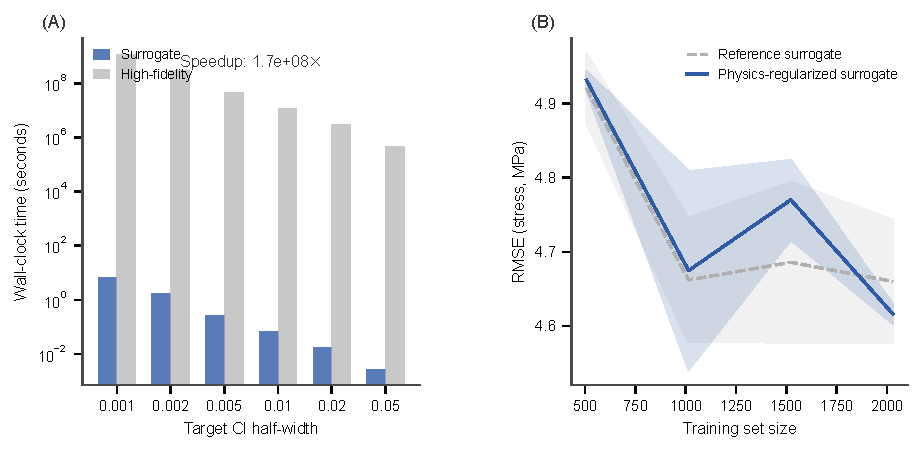
\includegraphics[width=\textwidth]{fig7_efficiency.pdf}
\caption{\textbf{Computational efficiency. / 计算效率。}
(\textbf{A})~Speedup of BNN surrogate relative to coupled HF solver:
single posterior-predictive draw ($1.43 \times 10^{5}\times$) and
batched per-sample inference ($1.37 \times 10^{8}\times$).
BNN 代理相对于耦合 HF 求解器的加速比。
(\textbf{B})~Data efficiency: per-output $R^2$ as a function of
training fraction (Supplementary Note~G).
数据效率：各输出 $R^2$ 随训练比例的变化（补充说明~G）。}
\label{fig:efficiency}
\end{figure}

\subsection{Limitations / 局限性}

The surrogate is trained on data from a single HPR design point. All
quantitative results describe this specific configuration only; a
different geometry, fuel enrichment or operating envelope would require
regenerating the training set and retraining the BNN. The methodology
itself is not design-specific: the same workflow of coupled-data
generation, BNN training and three-stage probabilistic analysis is
directly applicable to other reactor types and other coupled
multi-physics systems.

代理仅在单一 HPR 设计点的数据上训练，所有定量结果仅描述该构型。不同
几何、燃料富集度或运行工况需要重新生成训练集并重训 BNN。但方法本身
不依赖于特定设计：耦合数据生成、BNN 训练与三阶段概率分析的同一工作流
可直接应用于其他堆型和其他耦合多物理系统。

The MCMC calibration fixes four parameters (\Eslope{}, \Tref{},
\kslope{}, $\nu$) at their true values and calibrates the remaining
four. Extending to a full eight-parameter calibration would require
additional independent observations to constrain the expanded parameter
space. The reported posterior contraction is therefore conditional on
this four-parameter scope and should not be directly extrapolated to the
unconstrained eight-dimensional case.

MCMC 标定将四个参数（\Eslope{}、\Tref{}、\kslope{}、$\nu$）固定在
真实值上，对其余四个参数进行标定。扩展到完整八参数标定需要额外的
独立观测来约束扩展的参数空间。所报告的后验收缩量以四参数标定为前提，
不应直接外推到无约束的八维情形。

The \keff{} surrogate degrades on out-of-distribution feature-tail
subsets: on the \abase{} tail, \keff{} $R^2$ drops to ${\approx}0.31$
versus 0.849 in-distribution, while stress retains $R^2 \geq 0.93$
across all tested tails. The Sobol and posterior conclusions for \keff{}
therefore hold only within the training range of the dominant reactivity
parameter (Supplementary Fig.~S4).

\keff{} 代理在分布外特征尾部子集上退化：\abase{} 尾部 \keff{} $R^2$
降至约 0.31，分布内为 0.849；应力在所有尾部子集上均保持 $R^2 \geq 0.93$。
因此 \keff{} 的 Sobol 与后验结论仅在主控反应性参数的训练范围内成立
（补充图~S4）。

All posterior summaries in Section~2.5 are computed on the surrogate
side. An independent high-fidelity re-evaluation at the posterior-mean
parameter vectors (Supplementary Note~J; 18 cases $\times$ 3 posterior
labels = 54 HF runs) confirms consistency: stress MAE at the posterior
mean is 5.65\,MPa (4.5\% relative) and the [5\%, 95\%] HF envelope
covers all 18 true stress values. The present study uses synthetic
observations constructed from the high-fidelity solver because no real
operational data are available for this design. If experimental or
monitoring data become available in the future, the same posterior
calibration workflow can ingest real observations directly.

第~2.5 节的所有后验汇总量均在代理侧计算。在后验均值参数处对耦合求解器
的独立高保真重评估（补充说明~J；18 案例 $\times$ 3 后验标签 = 54 次
HF 运行）确认了一致性：后验均值处应力 MAE 为 5.65\,MPa（相对误差
4.5\%），[5\%, 95\%] HF 包络覆盖全部 18 个真实应力值。本研究使用由
高保真求解器构造的合成观测，因为该设计尚无真实运行数据。若未来获取
实验或监测数据，同一后验标定工作流可直接接入真实观测。

% ======================================================================
\section{Conclusion / 结论}
% ======================================================================

This work demonstrates that a single BNN posterior predictive
distribution can serve as the shared probabilistic layer on which
forward propagation, sensitivity attribution and posterior calibration
all operate---without retraining or recalibration between analyses.
Applied to a coupled OpenMC--FEniCS heat-pipe reactor model, the
framework yields three linked findings. First, forward Monte Carlo
propagation shows that two-way coupling damps stress variability by
${\approx}30\%$ relative to a decoupled prediction---a reduction
invisible to single-physics analyses. Second, Sobol decomposition
reveals that stress and \keff{} are governed by largely separate
parameter groups (\Eint{} and \abase{}, respectively), so the two
observables carry non-redundant information for inverse analysis. Third,
MCMC calibration contracts the material-parameter distribution toward
observation-compatible regions with 90\%-CI coverage 0.861 across 18
held-out benchmarks, and the posterior-mean BNN stress tracks the true
high-fidelity stress at MAE 10.4\,MPa over the 102--198\,MPa range.

本文表明，单一 BNN 后验预测分布可作为前向传播、敏感性归因与后验标定
三类分析共同依赖的概率层，且三者之间无需各自重训或重新校准。将该框架
应用于热管冷却反应堆的耦合 OpenMC--FEniCS 模型，得出三项相互关联的
发现。其一，前向蒙特卡洛传播表明双向耦合使应力变异相对解耦预测降低
约 30\%——单物理分析无法观测到这一降低。其二，Sobol 分解揭示应力与
\keff{} 分别由 \Eint{} 与 \abase{} 主导，两类观测量在反演中提供互补
信息。其三，MCMC 标定在 18 个基准案例上将材料参数分布收敛至与观测
相容的区域，90\%-CI 覆盖率为 0.861，后验均值 BNN 应力与真实高保真应力
的 MAE 为 10.4\,MPa，覆盖 102--198\,MPa 应力范围。

The surrogate is roughly five orders of magnitude cheaper per evaluation
than a coupled high-fidelity solve. This cost reduction makes the full
uncertainty workflow---propagation, sensitivity and calibration---executable
end-to-end on a single workstation. More broadly, the posterior-predictive
framework converts analyses that were previously gated by repeated
high-fidelity solves into routine computations on the same probabilistic
object. The workflow is not specific to this reactor design: any coupled
multi-physics system for which a BNN surrogate can be trained admits the
same three-stage analysis pipeline.

代理单次评估的代价较耦合高保真求解低约五个数量级。这一代价下降使
完整的不确定性工作流——传播、敏感性与标定——可在单台工作站上端到端
运行。更一般地，后验预测框架将原本受制于反复高保真求解的分析转变为在
同一概率对象上的常规计算。该工作流不局限于本堆型：任何能够训练 BNN
代理的耦合多物理系统均可采用同一三阶段分析流程。

% ======================================================================
\section{Methods / 方法}
% ======================================================================

\subsection{Material uncertainty model / 材料不确定性模型}

The coupled HPR simulation involves eight material properties of the
SS316 monolith grouped by physical function: structural mechanics
(\Eint{}, \Eslope{}, $\nu$), thermal deformation (\abase{}, \aslope{}),
and thermal transport (\kref{}, \Tref{}, \kslope{}). All eight are
assigned independent uniform priors with half-width 10\% of the nominal
design value. The same prior distribution is used throughout: as the
sampling distribution in forward UQ, as the input domain for Sobol
analysis, and as the prior in posterior calibration. Full parameter
definitions, nominal values and constitutive-law relationships are in
Supplementary Note~E and Supplementary Table~S1.

耦合 HPR 仿真涉及 SS316 一体化结构的八个材料属性，按物理功能分组：
结构力学（\Eint{}、\Eslope{}、$\nu$）、热变形（\abase{}、\aslope{}）
和热输运（\kref{}、\Tref{}、\kslope{}）。八个参数均赋予独立均匀先验，
半宽为标称设计值的 10\%。同一先验分布贯穿始终：作为前向 UQ 的采样分布、
Sobol 分析的输入域以及后验标定的先验。完整参数定义、标称值和本构关系见
补充说明~E 和补充表~S1。

\subsection{Coupled high-fidelity simulation / 耦合高保真仿真}

The high-fidelity workflow couples OpenMC Monte Carlo neutronics with the
FEniCS finite-element solver through a Picard fixed-point iteration
scheme\textsuperscript{9}. Two fidelity levels are retained: a decoupled
single-pass prediction before coupling convergence and a coupled
steady-state prediction after full convergence. Each HF evaluation
produces 15 scalar outputs. A dataset of $n = 3418$ samples was
generated by Latin hypercube sampling; samples were split into training
(2339), validation (501) and test (501) sets with a fixed random seed
(seed $= 2026$). The BNN maps directly from the 8 input parameters to
the 15 outputs without resolving intermediate coupling fields. Details
of the iteration scheme, convergence criteria and output definitions are
in Supplementary Note~E.

高保真工作流通过 Picard 不动点迭代格式耦合 OpenMC Monte Carlo 中子学
与 FEniCS 有限元求解器\textsuperscript{9}。保留两个保真度水平：耦合
收敛前的解耦单次预测和完全收敛后的耦合稳态预测。每次高保真评估产生
15 个标量输出。通过拉丁超立方采样生成 $n = 3418$ 的数据集；样本以固定
随机种子（seed $= 2026$）分为训练集（2339）、验证集（501）和测试集（501）。
BNN 直接从 8 个输入参数映射到 15 个输出，不解析中间耦合场。迭代格式、
收敛准则和输出定义详见补充说明~E。

\subsection{Bayesian neural network surrogate / 贝叶斯神经网络代理}

The surrogate is a BNN with mean-field variational inference (MFVI,
Bayes-by-Backprop\textsuperscript{10}). The network uses a fully
connected backbone with two output heads: a mean head and a log-variance
head that models heteroscedastic observation noise. Training minimises
the negative evidence lower bound (ELBO). The posterior predictive
distribution at a new input is approximated by Monte Carlo averaging
over $M$ weight samples from the trained variational posterior: at
inference $M = 50$, for Sobol analysis $M = 30$, and for the MCMC
likelihood $M = 20$. Hyperparameters were optimised via Optuna
(Supplementary Table~S2). Physics-prior monotonicity constraints are
incorporated as an auxiliary loss term during training. Full ELBO
derivation, KL annealing schedule and architecture details are in
Supplementary Note~A.

代理为采用均场变分推断（MFVI，Bayes-by-Backprop\textsuperscript{10}）
的 BNN。网络使用全连接骨干，带两个输出头：均值头和建模异方差观测噪声
的对数方差头。训练最小化负证据下界（ELBO）。新输入处的后验预测分布通过
对训练后变分后验的 $M$ 次权重采样进行 Monte Carlo 平均来近似：推理时
$M = 50$，Sobol 分析时 $M = 30$，MCMC 似然计算时 $M = 20$。超参数通过
Optuna 优化（补充表~S2）。物理先验单调性约束作为辅助损失项在训练中引入。
完整 ELBO 推导、KL 退火策略和架构细节见补充说明~A。

\subsection{Forward uncertainty propagation / 前向不确定性传播}

Forward UQ draws $N = 20{,}000$ Latin hypercube samples from the joint
prior and evaluates the BNN posterior predictive mean at each sample.
Using the predictive mean rather than a full predictive draw isolates
parametric uncertainty from the BNN's own epistemic and aleatoric spread;
the predictive-draw variant is reported in Supplementary Note~D.

前向 UQ 从联合先验中抽取 $N = 20{,}000$ 个拉丁超立方样本，并在每个样本
处评估 BNN 后验预测均值。使用预测均值而非完整预测抽样可将参数不确定性
与 BNN 自身的认知和随机展幅隔离；预测抽样变体在补充说明~D 中报告。

\subsection{Sobol sensitivity analysis / Sobol 敏感性分析}

Global sensitivity is assessed through variance-based Sobol indices
estimated with the Saltelli cross-matrix scheme ($N_S = 4096$ per
matrix, 40,960 surrogate evaluations per replication). The analysis is
repeated 50 times; a factor is treated as a stable contributor only if
the lower bound of its 90\% CI exceeds zero. Methodological details
including the Jansen estimator definition are in Supplementary Note~B.

全局敏感性通过基于方差的 Sobol 指标评估，采用 Saltelli 交叉矩阵方案
（每矩阵 $N_S = 4096$，每次重复 40,960 次代理评估）。分析重复 50 次；
仅当因素的 90\% CI 下界超过零时，才将其视为稳定贡献因素。方法细节
（包括 Jansen 估计量定义）见补充说明~B。

\subsection{Posterior calibration / 后验标定}

Posterior calibration uses Bayesian inference:
$p(\boldsymbol{\theta} \mid \mathbf{y}_{\mathrm{obs}}) \propto
p(\mathbf{y}_{\mathrm{obs}} \mid \boldsymbol{\theta})\,
\pi(\boldsymbol{\theta})$, with the likelihood evaluated through the BNN
posterior predictive mean. Four parameters are calibrated (\Eint{},
\abase{}, \aslope{}, \kref{}), selected on the basis of their Sobol
ranking; the remaining four are fixed at their true values. The 18
benchmark cases are drawn from the test split (6 low, 6 near, 6 high
stress). Observations are the true HF outputs of 5 primary coupled
quantities perturbed by 2\% multiplicative Gaussian noise. The posterior
is sampled by Metropolis--Hastings MCMC with 4 independent chains (8000
iterations, burn-in 2000, thinning 5). Implementation details and
convergence diagnostics are in Supplementary Note~C.

后验标定采用贝叶斯推断：
$p(\boldsymbol{\theta} \mid \mathbf{y}_{\mathrm{obs}}) \propto
p(\mathbf{y}_{\mathrm{obs}} \mid \boldsymbol{\theta})\,
\pi(\boldsymbol{\theta})$，似然通过 BNN 后验预测均值评估。标定四个
参数（\Eint{}、\abase{}、\aslope{}、\kref{}），基于其 Sobol 排名
选取；其余四个参数固定为真实值。18 个基准算例取自测试集（低应力 6 例、
阈值附近 6 例、高应力 6 例）。观测为 5 个主要耦合量的真实高保真输出加
2\% 乘性高斯噪声。后验通过 Metropolis--Hastings MCMC 采样，含 4 条独立链
（8000 次迭代，预热 2000 次，稀疏化步长 5）。实现细节和收敛诊断见
补充说明~C。

% ======================================================================
\section*{Data availability / 数据可用性}
% ======================================================================

The coupled simulation dataset and fixed train/validation/test split
used in this study are available at [repository URL upon acceptance].

本研究使用的耦合仿真数据集及固定的训练/验证/测试划分可通过
[接受后提供仓库 URL] 获取。

\section*{Code availability / 代码可用性}

The BNN training, evaluation and analysis code are available at
[repository URL upon acceptance].

BNN 训练、评估和分析代码可通过 [接受后提供仓库 URL] 获取。

% ======================================================================
\section*{References / 参考文献}
% ======================================================================

\begin{enumerate}\small
\item McClure PR, Poston DI, Dixon DD, Cooley JW. Design of megawatt
      power level heat pipe reactors. LANL, LA-UR-15-28840; 2015.
\item Stauff NE, et al. High-fidelity multiphysics modeling of a heat
      pipe microreactor using BlueCrab. \textit{Nucl.\ Sci.\ Eng.} 2024.
\item Miao Y, et al. Multiphysics simulation of KRUSTY warm critical
      experiments using MOOSE tools. \textit{Nucl.\ Sci.\ Eng.} 2025.
\item Aldebie F, et al. Thermal-mechanical safety analysis of heat pipe
      micro reactor. \textit{Nucl.\ Eng.\ Des.} 2024;420:113003.
\item Jeong MJ, et al. Multiphysics analysis of heat pipe cooled
      microreactor core. \textit{Front.\ Energy Res.} 2023;11:1213000.
\item Slaughter AE, et al. MOOSE Stochastic Tools. \textit{SoftwareX}.
      2023;22:101345.
\item Dhulipala SLN, et al. MOOSE ProbML. \textit{J.\ Comput.\ Sci.}
      2026;94:102776.
\item Lim JY, et al. A hybrid surrogate modeling framework for the
      Digital Twin of a FHR. \textit{Nucl.\ Eng.\ Des.} 2025;433:113690.
\item Zhang T, Chen Y, Wang S, Liu X. Design-oriented multiphysics
      analysis and surrogate modelling of a heat-pipe-cooled reactor.
      \textit{Energy}. 2025. (in press)
\item Blundell C, et al. Weight uncertainty in neural networks. ICML
      2015; pp.\ 1613--1622.
\item DOE Office of Nuclear Energy. What is a microreactor? 2021.
\item NASA. Fission Surface Power. 2024.
\item IEA. Electricity 2025: Analysis and forecast to 2027. Jan 2025.
\end{enumerate}

% ======================================================================
\section*{Acknowledgements / 致谢}
% ======================================================================

This research is supported by the National Natural Science Foundation
of China [12175138, 12427811]; Shanghai Rising-Star Program; and
LingChuang Research Project of China National Nuclear Corporation.

本研究获得国家自然科学基金 [12175138, 12427811]、上海市启明星计划和
中国核工业集团凌创研究项目的支持。

% ======================================================================
\section*{Author contributions / 作者贡献}
% ======================================================================

\textbf{CRediT authorship contribution statement}

\textbf{Yinuo Chen:} Writing -- original draft, Visualization, Software,
Methodology, Investigation, Formal analysis, Data curation.
\textbf{Sicheng Wang:} Writing -- review \& editing.
\textbf{Xiaojing Liu:} Writing -- review \& editing, Project
administration, Funding acquisition.
\textbf{Tengfei Zhang:} Writing -- review \& editing, Writing -- original
draft, Visualization, Supervision, Conceptualization, Project
administration, Funding acquisition.

\textbf{CRediT 作者贡献声明}

陈一诺：撰写——初稿，可视化，软件，方法学，调研，形式分析，数据整理。
王思成：撰写——审阅与修改。
刘晓晶：撰写——审阅与修改，项目管理，经费获取。
张腾飞：撰写——审阅与修改，撰写——初稿，可视化，指导，概念构思，
项目管理，经费获取。

% ======================================================================
\section*{Competing interests / 利益冲突声明}
% ======================================================================

The authors declare no competing interests.

作者声明不存在利益冲突。

\end{document}
